\PassOptionsToPackage{unicode=true}{hyperref} % options for packages loaded elsewhere
\PassOptionsToPackage{hyphens}{url}
\documentclass[11pt,dvipsnames,ignorenonframetext,aspectratio=169]{beamer}
\IfFileExists{pgfpages.sty}{\usepackage{pgfpages}}{}
\setbeamertemplate{caption}[numbered]
\setbeamertemplate{caption label separator}{: }
\setbeamercolor{caption name}{fg=normal text.fg}
\beamertemplatenavigationsymbolsempty
\usepackage{lmodern}
\usepackage{amssymb,amsmath}
\usepackage{ifxetex,ifluatex}
\usepackage{fixltx2e} % provides \textsubscript
\ifnum 0\ifxetex 1\fi\ifluatex 1\fi=0 % if pdftex
  \usepackage[T1]{fontenc}
  \usepackage[utf8]{inputenc}
\else % if luatex or xelatex
  \ifxetex
    \usepackage{mathspec}
  \else
    \usepackage{fontspec}
\fi
\defaultfontfeatures{Ligatures=TeX,Scale=MatchLowercase}







\fi

  \usetheme[]{monash}

  \usecolortheme{monashwhite}


% A default size of 24 is set in beamerthememonash.sty

% Title page
\setbeamertemplate{title page}
{\placefig{-0.01}{-0.01}{width=1.01\paperwidth,height=1.01\paperheight}{sissooleafwaterdrops.jpg}
\begin{textblock}{7.5}(1,2.8)\usebeamerfont{title}
{\color{white}\raggedright\par\inserttitle}
\end{textblock}
\begin{textblock}{7.5}(1,7)
{\color{white}\raggedright{\insertauthor}\mbox{}\\[0.2cm]
\insertdate}
\end{textblock}}


  \useinnertheme{rounded}

  \useoutertheme{smoothtree}

% use upquote if available, for straight quotes in verbatim environments
\IfFileExists{upquote.sty}{\usepackage{upquote}}{}
% use microtype if available
\IfFileExists{microtype.sty}{%
  \usepackage{microtype}
  \UseMicrotypeSet[protrusion]{basicmath} % disable protrusion for tt fonts
}{}


\newif\ifbibliography


\hypersetup{
      pdftitle={Crop discrimination, crop cutting, yield monitoring, soil mapping},
            colorlinks=true,
    linkcolor=red,
    citecolor=Blue,
    urlcolor=lightgrayd,
    breaklinks=true}
%\urlstyle{same}  % Use monospace font for urls







% Prevent slide breaks in the middle of a paragraph:
\widowpenalties 1 10000
\raggedbottom

  \AtBeginPart{
    \let\insertpartnumber\relax
    \let\partname\relax
    \frame{\partpage}
  }
  \AtBeginSection{
    \ifbibliography
    \else
      \let\insertsectionnumber\relax
      \let\sectionname\relax
      \frame{\sectionpage}
    \fi
  }
  \AtBeginSubsection{
    \let\insertsubsectionnumber\relax
    \let\subsectionname\relax
    \frame{\subsectionpage}
  }



\setlength{\parindent}{0pt}
\setlength{\parskip}{6pt plus 2pt minus 1pt}
\setlength{\emergencystretch}{3em}  % prevent overfull lines
\providecommand{\tightlist}{%
  \setlength{\itemsep}{0pt}\setlength{\parskip}{0pt}}

  \setcounter{secnumdepth}{0}


%% Monash overrides
\AtBeginSection[]{
   \frame<beamer>{
   \frametitle{Outline}\vspace*{0.2cm}
   
   \tableofcontents[currentsection,hideallsubsections]
  }}

% Redefine shaded environment if it exists (to ensure text is black)
\ifcsname Shaded\endcsname
  \definecolor{shadecolor}{RGB}{225,225,225}
  \renewenvironment{Shaded}{\color{black}\begin{snugshade}\color{black}}{\end{snugshade}}
\fi
%%


  \usepackage{setspace}
  \usepackage{wasysym}
  % \usepackage{footnote} % don't use this this breaks all
  \usepackage{fontenc}
  \usepackage{fontawesome}
  \usepackage{booktabs,siunitx}
  \usepackage{longtable}
  \usepackage{array}
  \usepackage{multirow}
  \usepackage{wrapfig}
  \usepackage{float}
  \usepackage{colortbl}
  \usepackage{pdflscape}
  \usepackage{tabu}
  \usepackage{threeparttable}
  \usepackage{threeparttablex}
  \usepackage[normalem]{ulem}
  \usepackage{makecell}
  \usepackage{xcolor}
  \usepackage{tikz} % required for image opacity change
  \usepackage[absolute,overlay]{textpos} % for text formatting
  \usepackage{chemfig}
  \usepackage[skip=0.333\baselineskip]{caption}
  % \newcommand*{\AlignChar}[1]{\makebox[1ex][c]{\ensuremath{\scriptstyle#1}}}%

  % this font option is amenable for beamer
  \setbeamerfont{caption}{size=\tiny}
  \singlespacing
  \definecolor{lightgrayd}{gray}{0.95}
  \definecolor{skyblued}{rgb}{0.65, 0.6, 0.94}
  \definecolor{oranged}{RGB}{245, 145, 200}

  % \newlength{\cslhangindent}
  % \setlength{\cslhangindent}{1.5em}
  % \newenvironment{cslreferences}%
  %   {\setlength{\parindent}{0pt}%
  %   \everypar{\setlength{\hangindent}{\cslhangindent}}\ignorespaces}%
  %   {\par}


  \newcommand{\bcolumns}{\begin{columns}[T, onlytextwidth]}
  \newcommand{\ecolumns}{\end{columns}}

  \newcommand{\bdescription}{\begin{description}}
  \newcommand{\edescription}{\end{description}}

  \newcommand{\bitemize}{\begin{itemize}}
  \newcommand{\eitemize}{\end{itemize}}
  \AtBeginSubsection{}

  \title[]{Crop discrimination, crop cutting, yield monitoring, soil
mapping}


  \author[
        \vspace{-0.5cm}Deependra Dhakal\\
Assistant Professor\\
\textit{ddhakal.rookie@gmail.com}\\
\url{https://rookie.rbind.io}
    ]{\vspace{-0.5cm}Deependra Dhakal\\
Assistant Professor\\
\textit{ddhakal.rookie@gmail.com}\\
\url{https://rookie.rbind.io}}


\date[
      
  ]{
    }

\begin{document}

% Hide progress bar and footline on titlepage
  \begin{frame}[plain]
  \titlepage
  \end{frame}


   \frame<beamer>{
   \frametitle{Outline}\vspace*{0.2cm}
   
   \tableofcontents[hideallsubsections]
  }

\hypertarget{crop-cutting}{%
\section{Crop cutting}\label{crop-cutting}}

\begin{frame}{Crop area and crop production assessment}
\protect\hypertarget{crop-area-and-crop-production-assessment}{}
\begin{itemize}
\tightlist
\item
  Information about crop area and production is crucial for planning of
  economic development initiatives, allocation of resources and
  monitoring the achievements
\item
  Area and production statistics has great importance for planners

  \begin{itemize}
  \tightlist
  \item
    preparation of national accounts of food crops
  \item
    decision making on export/import and price
  \item
    day to day management of the crop sector
  \end{itemize}
\item
  Statistical Information on Nepalese Agriculture (the annual
  agri-statistics publication) hosts acerage, crop production and basic
  farming household statistics.
\item
  The data collection is entrusted to extension staff, who carry out
  crop cut \alert{surveys} to assess crop yield.
\end{itemize}
\end{frame}

\begin{frame}{}
\protect\hypertarget{section}{}
\begin{itemize}
\tightlist
\item
  Crop cutting surveys are field surveys in which production data are
  collected through direct measurement for estimating yield of major
  field crops, paddy and wheat.
\item
  The technique was developed during 1940s and 1950s.
\item
  A \alert{plot} is \alert{randomly} selected of a given size in the
  field of a specific crop and its produce is harvested following
  specified methodology.
\item
  The harvested yield rate is calculated as the weight of the harvested
  crop divided by the area of the plot.
\end{itemize}

\[
\text{Estimated crop yield} = \frac{\text{Weight of harvest crop}}{\text{Area of the selected plot}}
\]
\end{frame}

\begin{frame}{Steps in Crop-cutting}
\protect\hypertarget{steps-in-crop-cutting}{}
\begin{itemize}
\tightlist
\item
  Selecting a field of mature crop ready for harvest
\item
  Identifying the south-west corner of field from where crop cut has to
  be done
\item
  Randomly demarcating the crop-cutting plot of a specified size
  (generally 10 or 20 msq)
\item
  Meticulously determining the plants to be included in the crop-cut
  plot
\item
  Harvesting of crop cut plot
\item
  Threshing and winnowing to get cleaned harvest
\item
  Weighing and adjusting the harvet to a specified level of moisture
  content
\item
  Converting the harvest to a standard unit, for example tons per
  hectare.
\end{itemize}
\end{frame}

\begin{frame}{Crop cutting survey design and selection}
\protect\hypertarget{crop-cutting-survey-design-and-selection}{}
\begin{itemize}
\tightlist
\item
  The design adopted in the survey is stratified multi-stage random
  sampling

  \begin{itemize}
  \tightlist
  \item
    Districts are taken as strata
  \item
    Specific local units (municipalities) are the first stage units
  \item
    Fields growing the crop under crop cutting experiments are the
    second stage units
  \item
    Experimental plots of specified size are the ultimate stage units
  \end{itemize}
\item
  In the strata, list of all villages with area growing the experimental
  crop is obtained
\item
  Generally in a district with 30 local units, 8-10 municipals are
  selected by SRS.
\item
  In field selection, agriculture technician proceeds to the selected
  village.

  \begin{itemize}
  \tightlist
  \item
    Cultivators are listed and serial number assigned to their fields
  \item
    Fields are selected by SRS
  \end{itemize}
\end{itemize}
\end{frame}

\begin{frame}{General considerations}
\protect\hypertarget{general-considerations}{}
\begin{itemize}
\tightlist
\item
  Area of selected field should be more than the total area of CCE plot.
\item
  The experimental crop in the field is not meant for seed production or
  demonstration.
\item
  If experimental crop is not germinated or has failed (cattle or pest
  damaged, affected by disease or heavy rainfall, inadequate rainfall),
  field is still considered for selection.
\item
  The crop cutting experiment should not be conducted in the selected
  field if a part or whole of the selected field has already been
  harvested.
\end{itemize}
\end{frame}

\begin{frame}{Locating of experimental plot}
\protect\hypertarget{locating-of-experimental-plot}{}
\begin{itemize}
\tightlist
\item
  Identification of south-west corner of the field (for consistency
  purpose in all surveys)
\item
  Start from SW corner of the field and measure in steps the length and
  breadth of the field
\item
  From the total number of steps of both length and breadth, deduct
  seven steps from each
\item
  Select experimental plot randomly (using a pair of random numbers to
  locate row-column combination)

  \begin{itemize}
  \tightlist
  \item
    for example, if the length is 86 steps, the remainder is 86-7 = 79
    and the breadth is 45 steps the remainder is 45-7 = 38
  \item
    select two random numbers one for length (\textless79) and other for
    breadth (\textless38)
  \item
    locate the plot based on selected pair of numbers, and fix a peg at
    that point.
  \end{itemize}
\end{itemize}
\end{frame}

\begin{frame}{Harvesting and yield estimation}
\protect\hypertarget{harvesting-and-yield-estimation}{}
\begin{itemize}
\tightlist
\item
  Harvested when crop is fully mature
\item
  Date is fixed by the field assistant in consultation with the
  cultivators concerned
\item
  Produce from the plot is harvested before the harvest of the entire
  field
\item
  Threshing, winnowing, weighing of the harvested produce and recording
  of green/fresh produce
\item
  Driage experiments are performed to get marketable form of produce
  from cultivating fields.

  \begin{itemize}
  \tightlist
  \item
    dry a fixed quantity of harvested produce (generally 1 kg) in the
    experimental plot by keeping the produce for a few days for drying
    and weighing the produce everyday till the weighings on two
    successive days reveal ``negligible'' reduction in weight
  \end{itemize}
\end{itemize}
\end{frame}

\begin{frame}{}
\protect\hypertarget{section-1}{}
\begin{itemize}
\tightlist
\item
  Weight of marketable produce of crop may be obtained by applying the
  moisture level recorded with the moisture meter to the normal level of
  moisture of the produce as per:
\end{itemize}

\[
\begin{aligned}
WG_{14\%} = FW \times \frac{100-MCG}{100-14} = FW \times \frac{100-20}{100-14}
\end{aligned}
\] where:

\footnotesize

\begin{itemize}
\tightlist
\item
  \(FW\) = Fresh weight,
\item
  \(MCG\) (in \%) = Moisture content of grain when fresh (say 20\%),
\item
  \(WG_{14}\) (in \%) = Weight of grain adjusted to 14\% moisture
  content.
\end{itemize}
\end{frame}

\begin{frame}{Requirements for crop cutting experiment}
\protect\hypertarget{requirements-for-crop-cutting-experiment}{}
\begin{itemize}
\tightlist
\item
  Measuring tape (\textasciitilde30m and above)
\item
  Weighing balance
\item
  Small gunny bags for driage experiment
\item
  Hessian cloth
\item
  Four straight, long bamboo pegs each of 1m length with spikes at one
  end and irron collars at the other end.
\item
  Record book
\end{itemize}
\end{frame}

\begin{frame}{Estimation}
\protect\hypertarget{estimation}{}
\begin{itemize}
\tightlist
\item
  In countries with regular agricultural reporting system, crop area
  (\(A\)) is obtained from records on complete enumeration basis.
\item
  Average crop yield (\(Y\)) is estimated by CCE on a sample basis.
\end{itemize}

\[
\text{Crop production} (P) = A \times Y
\]

\begin{itemize}
\tightlist
\item
  In countries where cadastral maps are available not no regular
  reporting system, both A and Y are estimated on the basis of sample
  surveys.
\item
  Usually large sample of villages (primary units) is selected for crop
  area estimation. This provides estimate of A
\item
  CCE are carried out in a sub-sample of the primary units selected for
  area enumeration. This provides estimate of \(Y\).
\end{itemize}
\end{frame}

\begin{frame}{Estimation}
\protect\hypertarget{estimation-1}{}
\begin{itemize}
\tightlist
\item
  Estimating yield from a district survey:

  \begin{itemize}
  \tightlist
  \item
    Number of stratum (s): \(S\)
  \item
    Area under the crop in the \(s^{th}\) stratum: \(a_s\)
  \item
    Number of villages (i): \(n_s\)
  \item
    Number of field (j) in the \(i^{th}\) village: \(n_{si}\)
  \item
    Experimental plot selected
  \end{itemize}
\end{itemize}
\end{frame}

\begin{frame}{}
\protect\hypertarget{section-2}{}
\small

If \(y_{sij}\) be the observed yield from the selected plot of the
\(j^{th}\) field of the \(i^{th}\) village of the \(s^{th}\) stratum,
then

Estimated average of green yield for the \(s^{th}\) stratum is:

\[
\small
\hat{\bar{Y}}_s^g = \frac{1}{n_s} \sum^{n_{s}}_{i = 1} \frac{1}{n_{si}} \sum^{n_{si}}_{j = 1} y_{sij}
\]

Estimate of the district level average yield of the dry marketable
produce per hectare is given by:

\[
\small
\hat{\bar{Y}}^m = d \times f \times \frac{\sum^S_{s = 1} a_s \hat{\bar{Y}}_s^g}{\sum^S_{s = 1}a_s}
\]

Where:

\begin{itemize}
\tightlist
\item
  d: driage ratio,
\item
  f: conversion factor for green yield to dry marketable produce per
  hectare i.e.~rice = 2/3 of paddy.
\end{itemize}
\end{frame}

\begin{frame}{Remote sensing for crop cut surveys}
\protect\hypertarget{remote-sensing-for-crop-cut-surveys}{}
\begin{itemize}
\tightlist
\item
  Utility of remote sensing data to identify areas under specific crops
  can be understood with following assessment:
\end{itemize}

``Any crop can be mapped with multispectral scanner data if, and only
if, the spectral values associated with the crop are detectably
different from the values of the other features to be mapped.''

\begin{itemize}
\tightlist
\item
  Concept of ``ground truth'' or reference data is essential to reliable
  identification of data.
\end{itemize}
\end{frame}

\hypertarget{cropvegetation-discrimination}{%
\section{Crop/vegetation
discrimination}\label{cropvegetation-discrimination}}

\begin{frame}{}
\protect\hypertarget{section-3}{}
\begin{itemize}
\tightlist
\item
  Cells in plant leaves effectively scatter light because of the high
  contrast in the index of refraction between water-rich cell contents
  and inter-cellular air spaces.
\item
  Plants that are engaged in photosynthesis use blue and red light as
  energy sources. They reflect little light back from these wavelengths.
\item
  The underlying principle for using NIR is that plants with different
  nutrient levels reflect light differently in specific wavelengths.
\end{itemize}
\end{frame}

\begin{frame}{Direct advantages}
\protect\hypertarget{direct-advantages}{}
\begin{itemize}
\tightlist
\item
  Fast and non-destructive,
\item
  Once calibrated correctly, reliably measures biophysical and
  biochemical vegetation variables
\item
  Covers a large spatial area at once
\item
  Temporal imaging helps analyze crop growth processes
\end{itemize}
\end{frame}

\begin{frame}{}
\protect\hypertarget{section-4}{}
\begin{itemize}
\tightlist
\item
  Researchers use portable spectroradiometer such as the PSR+ to study
  vegetation in-situ and confirm, modify, and better understand
  hyperspectral remote sensing data from satellites such as Sentinel, or
  plane flyovers.
\item
  By capturing and analyzing data such as leaf area index (LAI) and
  canopy chlorophyll content, vegetation can be modeled and compared to
  vegetation indices to reveal

  \begin{itemize}
  \tightlist
  \item
    health, stress, infestation, pollution, climate changes, drought,
    fertilization, etc.
  \end{itemize}
\item
  Following indices are used to describe the state of vegetation:

  \begin{itemize}
  \tightlist
  \item
    NDVI (Normalized Difference Vegetation Index),
  \item
    SR (Simple Ratio),
  \item
    SAVI (Soil Adjusted Vegetation Index),
  \item
    ARVI (Atmospherically Resistant Vegetation Index)
  \end{itemize}
\end{itemize}
\end{frame}

\begin{frame}{}
\protect\hypertarget{section-5}{}
\begin{figure}
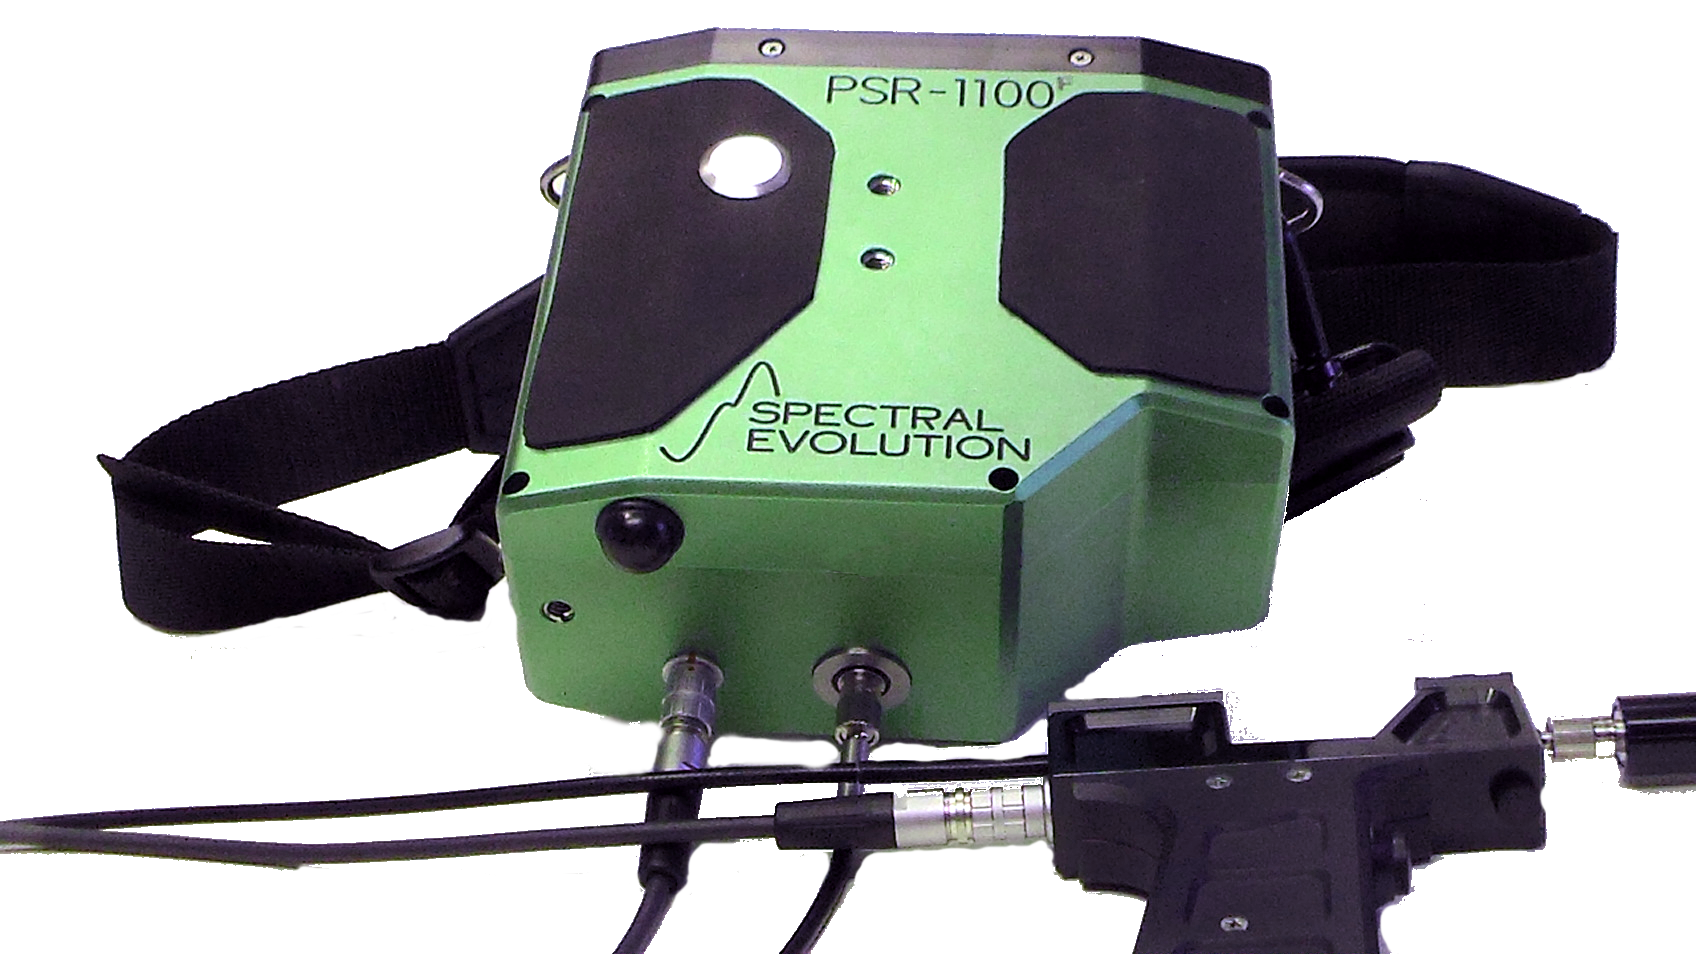
\includegraphics[width=0.45\linewidth]{../images/spectral_evolution_portable_spectroradiometer} \caption{PSR-1100f Spectral Evolution spectroradiometer commonly used in remote sensing of vegetation.}\label{fig:spectroradiometer}
\end{figure}
\end{frame}

\begin{frame}{}
\protect\hypertarget{section-6}{}
\begin{itemize}
\tightlist
\item
  Vegetation extraction from remote sensing imagery is the process of
  extracting vegetation information by interpreting satellite images
  based on the interpretation elements such as the image color, texture,
  tone, pattern and association information, etc.
\item
  Diverse methods (broadly grouped) either as supervised or as
  unsupervised depending on whether or not true ground data are inputted
  as references.
\item
  General steps involved in vegetation mapping include

  \begin{itemize}
  \tightlist
  \item
    image preprocessing (improve the quality of original images,
    highlighting the distinguishing features)
  \item
    image classification (results in the assignment of each pixel of the
    scene to one of the vegetation groups defined in a vegetation
    classification system or a membership matrix of the vegetation
    groups if fuzzy classification is adopted)
  \end{itemize}
\end{itemize}
\end{frame}

\begin{frame}{Normalized difference vegetation index}
\protect\hypertarget{normalized-difference-vegetation-index}{}
\begin{itemize}
\tightlist
\item
  NDVI is a simple graphical indicator that can be used to analyze
  remote sensing measurements, assessing whether or not the target being
  observed contains live green vegetation -- hence provides measurement
  of crop health.
\item
  Current research has proved that the NDVI images can even be obtained
  using the normal digital RGB cameras by some modifications in order to
  obtain the results similar to those obtained from the multispectral
  cameras
\item
  First normalized difference spectral index was formulated by Kriegler
  et al.~in 1969.
\item
  Rouse et al.~first applied the NDVI in the great plains in 1973.
\end{itemize}
\end{frame}

\begin{frame}{}
\protect\hypertarget{section-7}{}
\begin{itemize}
\tightlist
\item
  Green plants absorb solar radiation in the PAR spectral region and
  wavelengths longer than about 700 nm are too large to be used, hence
  reflected back.
\item
  Live green plants appear relatively dark in the PAR and relatively
  bright in the near-infrared
\item
  By contrast, clouds and snow tend to be rather bright in red (and
  visible wavelengths) and quite dark in the NIR.
\item
  Early instruments of Earth Observation, such as NASA's ERTS and NOAA'a
  AVHRR, acquired data in visible and near-infrared spectrum. Strong
  differences in plant reflectance was then used to determine their
  spatial distribution.
\end{itemize}
\end{frame}

\begin{frame}{}
\protect\hypertarget{section-8}{}
NDVI is calculated from these individual measurements as follows:

\[
NDVI = \frac{NIR - Red}{NIR + Red}
\]

where Red and NIR stand for the spectral reflectance measurements
acquired in the red (visible) and near-infrared regions, respectively.
These spectral reflectances are themselves ratios of the reflected
radiation to the incoming radiation in each spectral band individually,
hence they take on values between 0 and 1. By design, the NDVI itself
thus varies between -1 and +1.
\end{frame}

\begin{frame}{NDVI of Bagmati Province (April 25, 2022)}
\protect\hypertarget{ndvi-of-bagmati-province-april-25-2022}{}
\begin{center}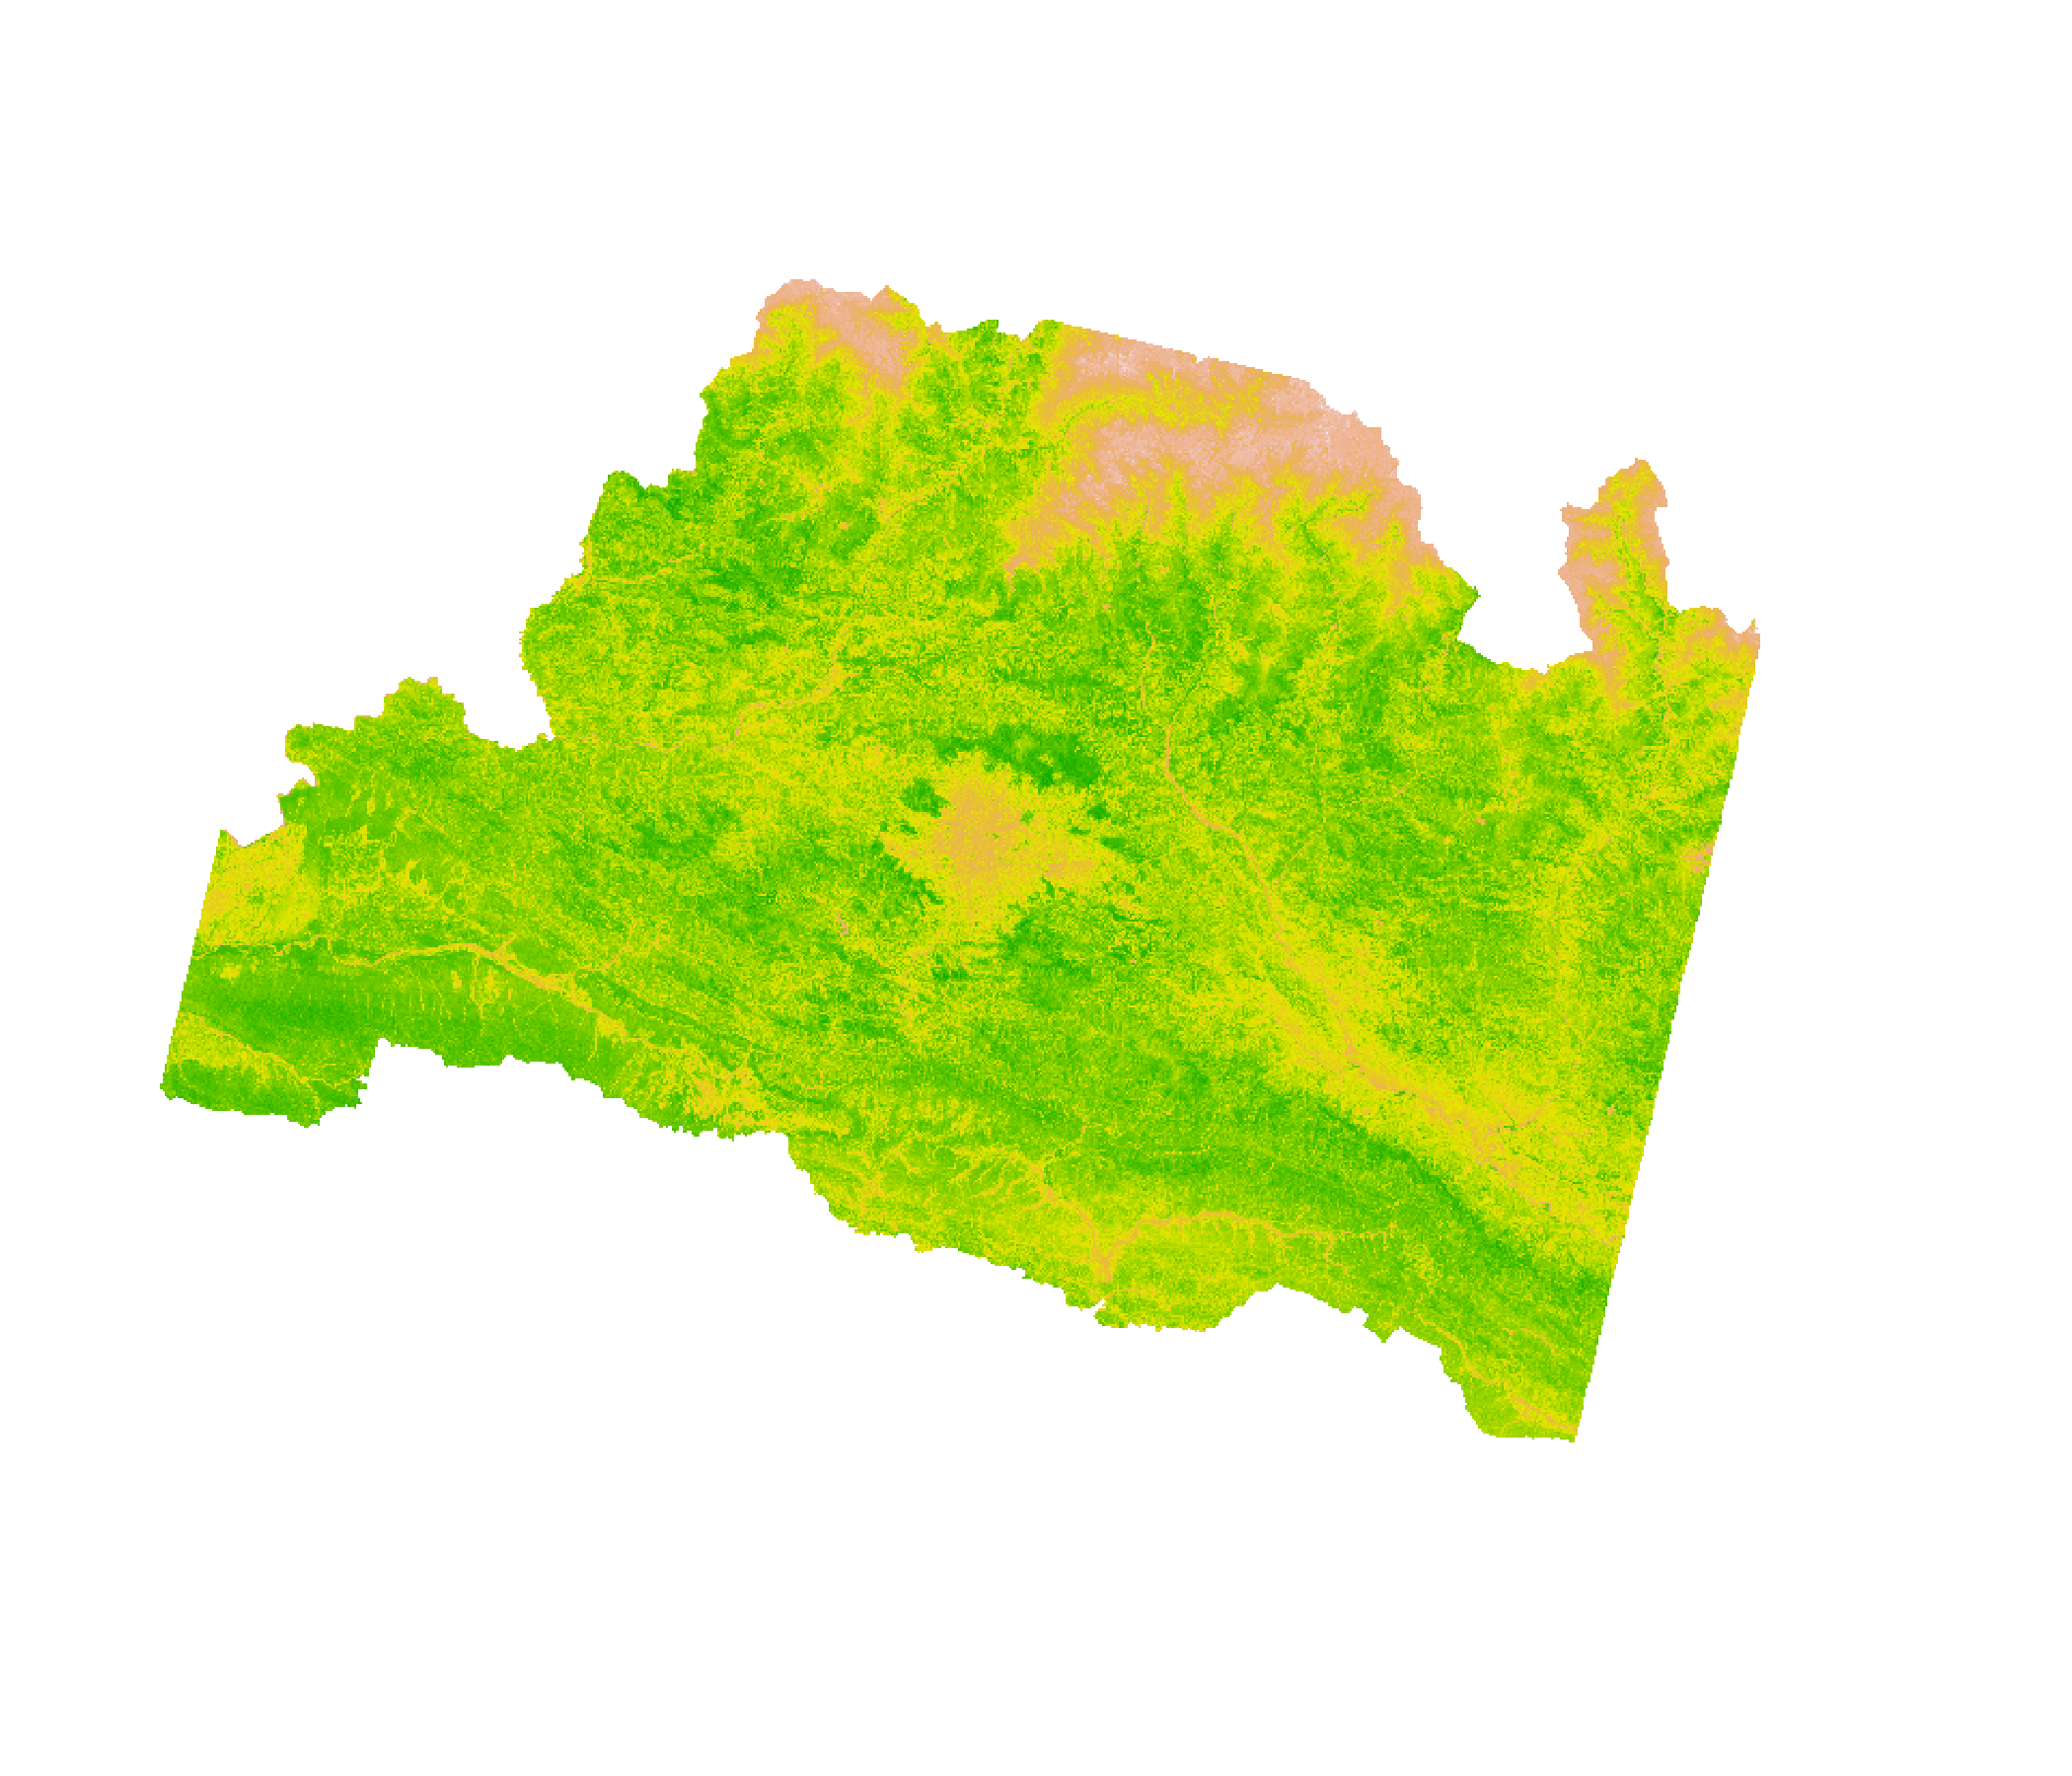
\includegraphics[width=0.7\linewidth]{../images/r_lc09_bagmati_raster_ndvi_value} \end{center}
\end{frame}

\begin{frame}{Practical -- NDVI (of Bagmati Province) calculation in
QGIS}
\protect\hypertarget{practical-ndvi-of-bagmati-province-calculation-in-qgis}{}
Refer to the qgis project file
``qgis\_bagmati\_province\_LC09\_raster,'' for use in calculation of
NDVI.
\end{frame}

\hypertarget{soil-mapping-and-fertilizer-recommendation}{%
\section{Soil mapping and fertilizer
recommendation}\label{soil-mapping-and-fertilizer-recommendation}}

\begin{frame}{}
\protect\hypertarget{section-9}{}
(Refer to the section on STCR in Lecture 1.)
\end{frame}

\hypertarget{bibliography}{%
\section{Bibliography}\label{bibliography}}

\begin{frame}{References}
\protect\hypertarget{references}{}
\end{frame}




\end{document}
